%% ECON 282E -- Session 4, Deck A1: Root-Finding -- Opening the Black Box
%% Discharges S03_A3's promise: "We build each of them -- bisection, secant,
%% Newton, Brent -- and their convergence rates, next week."
%% Frame budget deliberately exceeded across Session 4 (instructor's standing
%% instruction: content has priority, coverage decided in the room).
%% Every number from tools/figures/s04_numbers.json, keys "rootfinding",
%% "no_root", "systems", "damped_fixed_point".

%% ECON 282E -- Foundations of Macroeconomics (UC Riverside, Fall 2026)
%% Shared Beamer preamble for every deck in slides/S01 ... slides/S10.
%%
%% Usage (a deck lives in slides/S0X/ and is compiled from that folder):
%%   %% ECON 282E -- Foundations of Macroeconomics (UC Riverside, Fall 2026)
%% Shared Beamer preamble for every deck in slides/S01 ... slides/S10.
%%
%% Usage (a deck lives in slides/S0X/ and is compiled from that folder):
%%   %% ECON 282E -- Foundations of Macroeconomics (UC Riverside, Fall 2026)
%% Shared Beamer preamble for every deck in slides/S01 ... slides/S10.
%%
%% Usage (a deck lives in slides/S0X/ and is compiled from that folder):
%%   \input{../preamble/course_preamble.tex}
%%   \decktitle{1}{A1}{Who I Am \& Why This Course}{September 24, 2026}
%%   \begin{document}
%%   \makedecktitle
%%   ...
%%
%% Adapted from Courses/AI-ECON-2026/source/shared_preamble.tex (Metropolis theme,
%% concept/caution/example/takeaway boxes, \sectiondivider). Changes for this course:
%%   * course title block (\decktitle / \makedecktitle) instead of \makebeamertitle
%%   * \zh{...} typesets Chinese (book titles) under pdflatex via CJKutf8
%%   * researchbox for the "Research in the wild" frames
%%   * section pages off; TikZ libraries and the course map loaded here
%% Build with pdflatex only (two passes); tools/build_slides.py does this for you.

\documentclass[10pt,english,aspectratio=169]{beamer}

\usepackage[T1]{fontenc}
\usepackage{textcomp}
\usepackage[utf8]{inputenc}
\usepackage{babel}
\usepackage{CJKutf8}

\usepackage{amsmath, amssymb, amsthm, graphicx}
\usepackage{booktabs, multirow, tabularx}
\usepackage{tikz}
\usetikzlibrary{positioning,arrows.meta,shapes,calc,fit,backgrounds}
\usepackage{pgfplots}
\pgfplotsset{compat=1.16}
\usepackage[most]{tcolorbox}
\tcbuselibrary{skins, breakable}
\usepackage{listings}
\usepackage{xcolor}

\lstset{
  basicstyle=\ttfamily\small,
  keywordstyle=\color{blue!80!black}\bfseries,
  commentstyle=\color{green!50!black}\itshape,
  stringstyle=\color{orange!80!black},
  backgroundcolor=\color{gray!8},
  frame=single,
  rulecolor=\color{gray!40},
  breaklines=true,
  showstringspaces=false,
  numbers=none,
}

\usetheme{metropolis}
\usefonttheme{professionalfonts}
\metroset{sectionpage=none}

\definecolor{LightGray}{RGB}{230,230,230}
\definecolor{RedTitle}{RGB}{0,0,200}
\definecolor{VeryLightGray}{RGB}{245,245,245}
\definecolor{DarkText}{RGB}{0,0,0}
\definecolor{UCRBlue}{RGB}{0,45,106}
\definecolor{UCRGold}{RGB}{241,171,0}

% Stage colours of the course arc (used by the course map and elsewhere)
\colorlet{StageTrunk}{blue!12}
\colorlet{StageBranch}{cyan!14}
\colorlet{StageMachine}{gray!18}
\colorlet{StageWall}{red!14}
\colorlet{StageTools}{orange!20}
\colorlet{StageData}{green!16}
\colorlet{StageAgents}{violet!14}

\hypersetup{bookmarks=false,breaklinks=true,pdfborder={0 0 0},colorlinks=true,
  linkcolor=DarkText,urlcolor=RedTitle}

\setbeamercolor{background canvas}{bg=white}
\setbeamercolor{title}{fg=RedTitle}
\setbeamercolor{frametitle}{bg=VeryLightGray,fg=DarkText}
\setbeamercolor{normal text}{fg=DarkText}
\setbeamercolor{alerted text}{fg=RedTitle}
\setbeamersize{text margin left=5mm, text margin right=5mm}
\addtobeamertemplate{frametitle}{}{\vspace{-0.5em}}

\setbeamertemplate{navigation symbols}{}
\setbeamertemplate{footline}{%
  \hspace{5mm}{\usebeamerfont{page number in head/foot}\color{black!45}%
  ECON 282E \,$\cdot$\, \insertshortdeck}\hfill%
  \usebeamercolor[fg]{page number in head/foot}%
  \usebeamerfont{page number in head/foot}%
  \insertframenumber\,/\,\inserttotalframenumber\kern1em\vskip2pt%
}

% ---------------------------------------------------------------------------
% Chinese text under pdflatex (book titles etc.)
\newcommand{\zh}[1]{\begin{CJK*}{UTF8}{gbsn}#1\end{CJK*}}

% ---------------------------------------------------------------------------
% Deck title block
%   \decktitle{session}{deck id}{title}{date}
\newcommand{\insertshortdeck}{}
\newcommand{\decksession}{}
\newcommand{\deckid}{}
\newcommand{\decktitletext}{}
\newcommand{\deckdate}{}
\newcommand{\decktitle}[4]{%
  \renewcommand{\decksession}{#1}%
  \renewcommand{\deckid}{#2}%
  \renewcommand{\decktitletext}{#3}%
  \renewcommand{\deckdate}{#4}%
  \renewcommand{\insertshortdeck}{Session #1 \,$\cdot$\, Deck #1.#2}%
  \title{#3}%
  \author{Zhigang Feng}%
  \date{#4}%
}
\newcommand{\makedecktitle}{%
  \begin{frame}[plain,noframenumbering]
    \begin{tikzpicture}[remember picture,overlay]
      \fill[UCRBlue] (current page.north west) rectangle ([yshift=-0.55cm]current page.north east);
      \fill[UCRGold] ([yshift=-0.55cm]current page.north west) rectangle ([yshift=-0.62cm]current page.north east);
      \node[anchor=west, text=white, font=\small\bfseries] at ([xshift=5mm,yshift=-0.275cm]current page.north west)
        {ECON 282E \,$\cdot$\, Foundations of Macroeconomics};
      \node[anchor=east, text=white, font=\small] at ([xshift=-5mm,yshift=-0.275cm]current page.north east)
        {UC Riverside \,$\cdot$\, Fall 2026};
    \end{tikzpicture}
    \vspace*{1.1cm}
    {\usebeamerfont{title}\color{black!55}\large Session \decksession\ \,$\cdot$\, Deck \decksession.\deckid\par}
    \vspace{0.25cm}
    {\usebeamerfont{title}\color{RedTitle}\LARGE\bfseries \decktitletext\par}
    \vspace{0.7cm}
    {\large Zhigang Feng\par}
    \vspace{0.15cm}
    {\color{black!65}\deckdate\par}
    \vfill
    {\footnotesize\itshape\color{black!55}Build it on paper $\;\to\;$ solve it on the machine $\;\to\;$ push it to the frontier with AI\par}
  \end{frame}}

% ---------------------------------------------------------------------------
% Section divider (plain frame, not counted)
\newcommand{\sectiondivider}[2]{%
\begin{frame}[plain,noframenumbering]
\begin{center}
\vfill
{\Large\textbf{#1}\par}
\vspace{0.35cm}
{\normalsize #2\par}
\vfill
\end{center}
\end{frame}
}

% ---------------------------------------------------------------------------
% Boxes
\newtcolorbox{conceptbox}[1][]{colback=blue!3, colframe=RedTitle!55, boxrule=0.35mm,
  arc=1mm, left=2mm, right=2mm, top=1mm, bottom=1mm, #1}
\newtcolorbox{cautionbox}[1][]{colback=red!3, colframe=red!50!black, boxrule=0.35mm,
  arc=1mm, left=2mm, right=2mm, top=1mm, bottom=1mm, #1}
\newtcolorbox{examplebox}[1][]{colback=green!3, colframe=green!45!black, boxrule=0.35mm,
  arc=1mm, left=2mm, right=2mm, top=1mm, bottom=1mm, #1}
\newtcolorbox{takeawaybox}[1][]{colback=VeryLightGray, colframe=RedTitle!55, boxrule=0.35mm,
  arc=1mm, left=2mm, right=2mm, top=1mm, bottom=1mm, #1}
\newtcolorbox{researchbox}[1][]{enhanced, colback=violet!4, colframe=violet!60!black,
  boxrule=0.35mm, arc=1mm, left=2mm, right=2mm, top=1mm, bottom=1mm,
  fonttitle=\bfseries\small, title={Research in the wild}, #1}

\newcommand{\compacttables}{\renewcommand{\arraystretch}{1.15}}
\newcommand{\src}[1]{{\tiny\color{black!55}#1}}

% ---------------------------------------------------------------------------
\input{../preamble/course_map.tex}

%%   \decktitle{1}{A1}{Who I Am \& Why This Course}{September 24, 2026}
%%   \begin{document}
%%   \makedecktitle
%%   ...
%%
%% Adapted from Courses/AI-ECON-2026/source/shared_preamble.tex (Metropolis theme,
%% concept/caution/example/takeaway boxes, \sectiondivider). Changes for this course:
%%   * course title block (\decktitle / \makedecktitle) instead of \makebeamertitle
%%   * \zh{...} typesets Chinese (book titles) under pdflatex via CJKutf8
%%   * researchbox for the "Research in the wild" frames
%%   * section pages off; TikZ libraries and the course map loaded here
%% Build with pdflatex only (two passes); tools/build_slides.py does this for you.

\documentclass[10pt,english,aspectratio=169]{beamer}

\usepackage[T1]{fontenc}
\usepackage{textcomp}
\usepackage[utf8]{inputenc}
\usepackage{babel}
\usepackage{CJKutf8}

\usepackage{amsmath, amssymb, amsthm, graphicx}
\usepackage{booktabs, multirow, tabularx}
\usepackage{tikz}
\usetikzlibrary{positioning,arrows.meta,shapes,calc,fit,backgrounds}
\usepackage{pgfplots}
\pgfplotsset{compat=1.16}
\usepackage[most]{tcolorbox}
\tcbuselibrary{skins, breakable}
\usepackage{listings}
\usepackage{xcolor}

\lstset{
  basicstyle=\ttfamily\small,
  keywordstyle=\color{blue!80!black}\bfseries,
  commentstyle=\color{green!50!black}\itshape,
  stringstyle=\color{orange!80!black},
  backgroundcolor=\color{gray!8},
  frame=single,
  rulecolor=\color{gray!40},
  breaklines=true,
  showstringspaces=false,
  numbers=none,
}

\usetheme{metropolis}
\usefonttheme{professionalfonts}
\metroset{sectionpage=none}

\definecolor{LightGray}{RGB}{230,230,230}
\definecolor{RedTitle}{RGB}{0,0,200}
\definecolor{VeryLightGray}{RGB}{245,245,245}
\definecolor{DarkText}{RGB}{0,0,0}
\definecolor{UCRBlue}{RGB}{0,45,106}
\definecolor{UCRGold}{RGB}{241,171,0}

% Stage colours of the course arc (used by the course map and elsewhere)
\colorlet{StageTrunk}{blue!12}
\colorlet{StageBranch}{cyan!14}
\colorlet{StageMachine}{gray!18}
\colorlet{StageWall}{red!14}
\colorlet{StageTools}{orange!20}
\colorlet{StageData}{green!16}
\colorlet{StageAgents}{violet!14}

\hypersetup{bookmarks=false,breaklinks=true,pdfborder={0 0 0},colorlinks=true,
  linkcolor=DarkText,urlcolor=RedTitle}

\setbeamercolor{background canvas}{bg=white}
\setbeamercolor{title}{fg=RedTitle}
\setbeamercolor{frametitle}{bg=VeryLightGray,fg=DarkText}
\setbeamercolor{normal text}{fg=DarkText}
\setbeamercolor{alerted text}{fg=RedTitle}
\setbeamersize{text margin left=5mm, text margin right=5mm}
\addtobeamertemplate{frametitle}{}{\vspace{-0.5em}}

\setbeamertemplate{navigation symbols}{}
\setbeamertemplate{footline}{%
  \hspace{5mm}{\usebeamerfont{page number in head/foot}\color{black!45}%
  ECON 282E \,$\cdot$\, \insertshortdeck}\hfill%
  \usebeamercolor[fg]{page number in head/foot}%
  \usebeamerfont{page number in head/foot}%
  \insertframenumber\,/\,\inserttotalframenumber\kern1em\vskip2pt%
}

% ---------------------------------------------------------------------------
% Chinese text under pdflatex (book titles etc.)
\newcommand{\zh}[1]{\begin{CJK*}{UTF8}{gbsn}#1\end{CJK*}}

% ---------------------------------------------------------------------------
% Deck title block
%   \decktitle{session}{deck id}{title}{date}
\newcommand{\insertshortdeck}{}
\newcommand{\decksession}{}
\newcommand{\deckid}{}
\newcommand{\decktitletext}{}
\newcommand{\deckdate}{}
\newcommand{\decktitle}[4]{%
  \renewcommand{\decksession}{#1}%
  \renewcommand{\deckid}{#2}%
  \renewcommand{\decktitletext}{#3}%
  \renewcommand{\deckdate}{#4}%
  \renewcommand{\insertshortdeck}{Session #1 \,$\cdot$\, Deck #1.#2}%
  \title{#3}%
  \author{Zhigang Feng}%
  \date{#4}%
}
\newcommand{\makedecktitle}{%
  \begin{frame}[plain,noframenumbering]
    \begin{tikzpicture}[remember picture,overlay]
      \fill[UCRBlue] (current page.north west) rectangle ([yshift=-0.55cm]current page.north east);
      \fill[UCRGold] ([yshift=-0.55cm]current page.north west) rectangle ([yshift=-0.62cm]current page.north east);
      \node[anchor=west, text=white, font=\small\bfseries] at ([xshift=5mm,yshift=-0.275cm]current page.north west)
        {ECON 282E \,$\cdot$\, Foundations of Macroeconomics};
      \node[anchor=east, text=white, font=\small] at ([xshift=-5mm,yshift=-0.275cm]current page.north east)
        {UC Riverside \,$\cdot$\, Fall 2026};
    \end{tikzpicture}
    \vspace*{1.1cm}
    {\usebeamerfont{title}\color{black!55}\large Session \decksession\ \,$\cdot$\, Deck \decksession.\deckid\par}
    \vspace{0.25cm}
    {\usebeamerfont{title}\color{RedTitle}\LARGE\bfseries \decktitletext\par}
    \vspace{0.7cm}
    {\large Zhigang Feng\par}
    \vspace{0.15cm}
    {\color{black!65}\deckdate\par}
    \vfill
    {\footnotesize\itshape\color{black!55}Build it on paper $\;\to\;$ solve it on the machine $\;\to\;$ push it to the frontier with AI\par}
  \end{frame}}

% ---------------------------------------------------------------------------
% Section divider (plain frame, not counted)
\newcommand{\sectiondivider}[2]{%
\begin{frame}[plain,noframenumbering]
\begin{center}
\vfill
{\Large\textbf{#1}\par}
\vspace{0.35cm}
{\normalsize #2\par}
\vfill
\end{center}
\end{frame}
}

% ---------------------------------------------------------------------------
% Boxes
\newtcolorbox{conceptbox}[1][]{colback=blue!3, colframe=RedTitle!55, boxrule=0.35mm,
  arc=1mm, left=2mm, right=2mm, top=1mm, bottom=1mm, #1}
\newtcolorbox{cautionbox}[1][]{colback=red!3, colframe=red!50!black, boxrule=0.35mm,
  arc=1mm, left=2mm, right=2mm, top=1mm, bottom=1mm, #1}
\newtcolorbox{examplebox}[1][]{colback=green!3, colframe=green!45!black, boxrule=0.35mm,
  arc=1mm, left=2mm, right=2mm, top=1mm, bottom=1mm, #1}
\newtcolorbox{takeawaybox}[1][]{colback=VeryLightGray, colframe=RedTitle!55, boxrule=0.35mm,
  arc=1mm, left=2mm, right=2mm, top=1mm, bottom=1mm, #1}
\newtcolorbox{researchbox}[1][]{enhanced, colback=violet!4, colframe=violet!60!black,
  boxrule=0.35mm, arc=1mm, left=2mm, right=2mm, top=1mm, bottom=1mm,
  fonttitle=\bfseries\small, title={Research in the wild}, #1}

\newcommand{\compacttables}{\renewcommand{\arraystretch}{1.15}}
\newcommand{\src}[1]{{\tiny\color{black!55}#1}}

% ---------------------------------------------------------------------------
%% Course map: the recurring "you are here" slide for ECON 282E.
%% Loaded by course_preamble.tex. Pattern follows AI-ECON-2026 lec01_map.tex, but the map
%% shows the whole ten-session course rather than one lecture.
%%
%%   \CourseMap{s}{label}   s = 1..10 highlights session s and prints "you are here: label"
%%                          (e.g. \CourseMap{1}{1.A2}); earlier sessions get a check mark.
%%   \CourseMap{0}{}        full overview, nothing highlighted.
%%
%% Note: TikZ option lists are comma-split before TeX conditionals run, so every \ifnum
%% below sits outside [...] option lists.

\newcommand{\CourseMap}[2]{%
\begin{center}
\begin{tikzpicture}[
    sess/.style={rectangle, rounded corners=2pt, draw=black!45, minimum width=1.34cm,
        minimum height=1.12cm, text width=1.26cm, align=center, inner sep=1pt},
    stage/.style={font=\tiny\bfseries, text=black!70},
]
  \foreach \i/\d/\t/\c in {%
      1/Sep 24/Intro \\ Growth/StageTrunk,
      2/Oct 1/HA $\cdot$ OLG \\ Policy/StageBranch,
      3/Oct 8/Num.\ DP \\ Python/StageMachine,
      4/Oct 15/Numerics \\ I/StageMachine,
      5/Oct 22/Numerics \\ II/StageMachine,
      6/Oct 29/The wall \\ \textbf{Midterm}/StageWall,
      7/Nov 5/ML \\ Deep nets/StageTools,
      8/Nov 12/RL \\ HA $+$ DL/StageTools,
      9/Nov 19/Text \\ LLMs/StageData,
      10/Dec 3/Agents \\ \textbf{Projects}/StageAgents} {
    \node[sess, fill=\c] (n\i) at ({1.46*(\i-1)}, 0)
      {{\scriptsize\bfseries S\i}\\[-1pt]{\tiny\color{black!60}\d}\\[1pt]{\tiny \t}};
    \ifnum\i<#1
      \node[font=\scriptsize, text=green!45!black] at ([xshift=-2.5mm,yshift=-2.2mm]n\i.north east) {$\checkmark$};
    \fi
    \ifnum\i=#1
      \draw[RedTitle, very thick, rounded corners=2pt]
        ([xshift=-0.6mm,yshift=-0.6mm]n\i.south west) rectangle ([xshift=0.6mm,yshift=0.6mm]n\i.north east);
      % keep the label inside the picture at both ends of the row
      \ifnum\i<3
        \node[font=\scriptsize\bfseries, text=RedTitle, anchor=south west] at ([yshift=1.2mm]n\i.north west)
          {$\blacktriangledown$\,you are here: #2};
      \else\ifnum\i>8
        \node[font=\scriptsize\bfseries, text=RedTitle, anchor=south east] at ([yshift=1.2mm]n\i.north east)
          {you are here: #2\,$\blacktriangledown$};
      \else
        \node[font=\scriptsize\bfseries, text=RedTitle, anchor=south] at ([yshift=1.2mm]n\i.north)
          {you are here: #2\,$\blacktriangledown$};
      \fi\fi
    \fi
  }
  % stage band under the sessions
  \foreach \a/\b/\lab/\c in {1/1/trunk/StageTrunk, 2/2/branches/StageBranch,
      3/5/the machine $\cdot$ classical methods/StageMachine, 6/6/the wall/StageWall,
      7/8/new tools/StageTools, 9/9/new data/StageData, 10/10/colleagues/StageAgents} {
    \fill[\c] ([yshift=-1.5mm]n\a.south west) rectangle ([yshift=-4.6mm]n\b.south east);
    \path ([yshift=-1.5mm]n\a.south west) -- ([yshift=-4.6mm]n\b.south east)
      node[midway, stage] {\lab};
  }
  \node[font=\footnotesize\itshape, text=black!70] at ([yshift=-9.5mm]$(n1.south)!0.5!(n10.south)$)
    {Build it on paper $\;\to\;$ solve it on the machine $\;\to\;$ push it to the frontier with AI};
\end{tikzpicture}
\end{center}
}


%%   \decktitle{1}{A1}{Who I Am \& Why This Course}{September 24, 2026}
%%   \begin{document}
%%   \makedecktitle
%%   ...
%%
%% Adapted from Courses/AI-ECON-2026/source/shared_preamble.tex (Metropolis theme,
%% concept/caution/example/takeaway boxes, \sectiondivider). Changes for this course:
%%   * course title block (\decktitle / \makedecktitle) instead of \makebeamertitle
%%   * \zh{...} typesets Chinese (book titles) under pdflatex via CJKutf8
%%   * researchbox for the "Research in the wild" frames
%%   * section pages off; TikZ libraries and the course map loaded here
%% Build with pdflatex only (two passes); tools/build_slides.py does this for you.

\documentclass[10pt,english,aspectratio=169]{beamer}

\usepackage[T1]{fontenc}
\usepackage{textcomp}
\usepackage[utf8]{inputenc}
\usepackage{babel}
\usepackage{CJKutf8}

\usepackage{amsmath, amssymb, amsthm, graphicx}
\usepackage{booktabs, multirow, tabularx}
\usepackage{tikz}
\usetikzlibrary{positioning,arrows.meta,shapes,calc,fit,backgrounds}
\usepackage{pgfplots}
\pgfplotsset{compat=1.16}
\usepackage[most]{tcolorbox}
\tcbuselibrary{skins, breakable}
\usepackage{listings}
\usepackage{xcolor}

\lstset{
  basicstyle=\ttfamily\small,
  keywordstyle=\color{blue!80!black}\bfseries,
  commentstyle=\color{green!50!black}\itshape,
  stringstyle=\color{orange!80!black},
  backgroundcolor=\color{gray!8},
  frame=single,
  rulecolor=\color{gray!40},
  breaklines=true,
  showstringspaces=false,
  numbers=none,
}

\usetheme{metropolis}
\usefonttheme{professionalfonts}
\metroset{sectionpage=none}

\definecolor{LightGray}{RGB}{230,230,230}
\definecolor{RedTitle}{RGB}{0,0,200}
\definecolor{VeryLightGray}{RGB}{245,245,245}
\definecolor{DarkText}{RGB}{0,0,0}
\definecolor{UCRBlue}{RGB}{0,45,106}
\definecolor{UCRGold}{RGB}{241,171,0}

% Stage colours of the course arc (used by the course map and elsewhere)
\colorlet{StageTrunk}{blue!12}
\colorlet{StageBranch}{cyan!14}
\colorlet{StageMachine}{gray!18}
\colorlet{StageWall}{red!14}
\colorlet{StageTools}{orange!20}
\colorlet{StageData}{green!16}
\colorlet{StageAgents}{violet!14}

\hypersetup{bookmarks=false,breaklinks=true,pdfborder={0 0 0},colorlinks=true,
  linkcolor=DarkText,urlcolor=RedTitle}

\setbeamercolor{background canvas}{bg=white}
\setbeamercolor{title}{fg=RedTitle}
\setbeamercolor{frametitle}{bg=VeryLightGray,fg=DarkText}
\setbeamercolor{normal text}{fg=DarkText}
\setbeamercolor{alerted text}{fg=RedTitle}
\setbeamersize{text margin left=5mm, text margin right=5mm}
\addtobeamertemplate{frametitle}{}{\vspace{-0.5em}}

\setbeamertemplate{navigation symbols}{}
\setbeamertemplate{footline}{%
  \hspace{5mm}{\usebeamerfont{page number in head/foot}\color{black!45}%
  ECON 282E \,$\cdot$\, \insertshortdeck}\hfill%
  \usebeamercolor[fg]{page number in head/foot}%
  \usebeamerfont{page number in head/foot}%
  \insertframenumber\,/\,\inserttotalframenumber\kern1em\vskip2pt%
}

% ---------------------------------------------------------------------------
% Chinese text under pdflatex (book titles etc.)
\newcommand{\zh}[1]{\begin{CJK*}{UTF8}{gbsn}#1\end{CJK*}}

% ---------------------------------------------------------------------------
% Deck title block
%   \decktitle{session}{deck id}{title}{date}
\newcommand{\insertshortdeck}{}
\newcommand{\decksession}{}
\newcommand{\deckid}{}
\newcommand{\decktitletext}{}
\newcommand{\deckdate}{}
\newcommand{\decktitle}[4]{%
  \renewcommand{\decksession}{#1}%
  \renewcommand{\deckid}{#2}%
  \renewcommand{\decktitletext}{#3}%
  \renewcommand{\deckdate}{#4}%
  \renewcommand{\insertshortdeck}{Session #1 \,$\cdot$\, Deck #1.#2}%
  \title{#3}%
  \author{Zhigang Feng}%
  \date{#4}%
}
\newcommand{\makedecktitle}{%
  \begin{frame}[plain,noframenumbering]
    \begin{tikzpicture}[remember picture,overlay]
      \fill[UCRBlue] (current page.north west) rectangle ([yshift=-0.55cm]current page.north east);
      \fill[UCRGold] ([yshift=-0.55cm]current page.north west) rectangle ([yshift=-0.62cm]current page.north east);
      \node[anchor=west, text=white, font=\small\bfseries] at ([xshift=5mm,yshift=-0.275cm]current page.north west)
        {ECON 282E \,$\cdot$\, Foundations of Macroeconomics};
      \node[anchor=east, text=white, font=\small] at ([xshift=-5mm,yshift=-0.275cm]current page.north east)
        {UC Riverside \,$\cdot$\, Fall 2026};
    \end{tikzpicture}
    \vspace*{1.1cm}
    {\usebeamerfont{title}\color{black!55}\large Session \decksession\ \,$\cdot$\, Deck \decksession.\deckid\par}
    \vspace{0.25cm}
    {\usebeamerfont{title}\color{RedTitle}\LARGE\bfseries \decktitletext\par}
    \vspace{0.7cm}
    {\large Zhigang Feng\par}
    \vspace{0.15cm}
    {\color{black!65}\deckdate\par}
    \vfill
    {\footnotesize\itshape\color{black!55}Build it on paper $\;\to\;$ solve it on the machine $\;\to\;$ push it to the frontier with AI\par}
  \end{frame}}

% ---------------------------------------------------------------------------
% Section divider (plain frame, not counted)
\newcommand{\sectiondivider}[2]{%
\begin{frame}[plain,noframenumbering]
\begin{center}
\vfill
{\Large\textbf{#1}\par}
\vspace{0.35cm}
{\normalsize #2\par}
\vfill
\end{center}
\end{frame}
}

% ---------------------------------------------------------------------------
% Boxes
\newtcolorbox{conceptbox}[1][]{colback=blue!3, colframe=RedTitle!55, boxrule=0.35mm,
  arc=1mm, left=2mm, right=2mm, top=1mm, bottom=1mm, #1}
\newtcolorbox{cautionbox}[1][]{colback=red!3, colframe=red!50!black, boxrule=0.35mm,
  arc=1mm, left=2mm, right=2mm, top=1mm, bottom=1mm, #1}
\newtcolorbox{examplebox}[1][]{colback=green!3, colframe=green!45!black, boxrule=0.35mm,
  arc=1mm, left=2mm, right=2mm, top=1mm, bottom=1mm, #1}
\newtcolorbox{takeawaybox}[1][]{colback=VeryLightGray, colframe=RedTitle!55, boxrule=0.35mm,
  arc=1mm, left=2mm, right=2mm, top=1mm, bottom=1mm, #1}
\newtcolorbox{researchbox}[1][]{enhanced, colback=violet!4, colframe=violet!60!black,
  boxrule=0.35mm, arc=1mm, left=2mm, right=2mm, top=1mm, bottom=1mm,
  fonttitle=\bfseries\small, title={Research in the wild}, #1}

\newcommand{\compacttables}{\renewcommand{\arraystretch}{1.15}}
\newcommand{\src}[1]{{\tiny\color{black!55}#1}}

% ---------------------------------------------------------------------------
%% Course map: the recurring "you are here" slide for ECON 282E.
%% Loaded by course_preamble.tex. Pattern follows AI-ECON-2026 lec01_map.tex, but the map
%% shows the whole ten-session course rather than one lecture.
%%
%%   \CourseMap{s}{label}   s = 1..10 highlights session s and prints "you are here: label"
%%                          (e.g. \CourseMap{1}{1.A2}); earlier sessions get a check mark.
%%   \CourseMap{0}{}        full overview, nothing highlighted.
%%
%% Note: TikZ option lists are comma-split before TeX conditionals run, so every \ifnum
%% below sits outside [...] option lists.

\newcommand{\CourseMap}[2]{%
\begin{center}
\begin{tikzpicture}[
    sess/.style={rectangle, rounded corners=2pt, draw=black!45, minimum width=1.34cm,
        minimum height=1.12cm, text width=1.26cm, align=center, inner sep=1pt},
    stage/.style={font=\tiny\bfseries, text=black!70},
]
  \foreach \i/\d/\t/\c in {%
      1/Sep 24/Intro \\ Growth/StageTrunk,
      2/Oct 1/HA $\cdot$ OLG \\ Policy/StageBranch,
      3/Oct 8/Num.\ DP \\ Python/StageMachine,
      4/Oct 15/Numerics \\ I/StageMachine,
      5/Oct 22/Numerics \\ II/StageMachine,
      6/Oct 29/The wall \\ \textbf{Midterm}/StageWall,
      7/Nov 5/ML \\ Deep nets/StageTools,
      8/Nov 12/RL \\ HA $+$ DL/StageTools,
      9/Nov 19/Text \\ LLMs/StageData,
      10/Dec 3/Agents \\ \textbf{Projects}/StageAgents} {
    \node[sess, fill=\c] (n\i) at ({1.46*(\i-1)}, 0)
      {{\scriptsize\bfseries S\i}\\[-1pt]{\tiny\color{black!60}\d}\\[1pt]{\tiny \t}};
    \ifnum\i<#1
      \node[font=\scriptsize, text=green!45!black] at ([xshift=-2.5mm,yshift=-2.2mm]n\i.north east) {$\checkmark$};
    \fi
    \ifnum\i=#1
      \draw[RedTitle, very thick, rounded corners=2pt]
        ([xshift=-0.6mm,yshift=-0.6mm]n\i.south west) rectangle ([xshift=0.6mm,yshift=0.6mm]n\i.north east);
      % keep the label inside the picture at both ends of the row
      \ifnum\i<3
        \node[font=\scriptsize\bfseries, text=RedTitle, anchor=south west] at ([yshift=1.2mm]n\i.north west)
          {$\blacktriangledown$\,you are here: #2};
      \else\ifnum\i>8
        \node[font=\scriptsize\bfseries, text=RedTitle, anchor=south east] at ([yshift=1.2mm]n\i.north east)
          {you are here: #2\,$\blacktriangledown$};
      \else
        \node[font=\scriptsize\bfseries, text=RedTitle, anchor=south] at ([yshift=1.2mm]n\i.north)
          {you are here: #2\,$\blacktriangledown$};
      \fi\fi
    \fi
  }
  % stage band under the sessions
  \foreach \a/\b/\lab/\c in {1/1/trunk/StageTrunk, 2/2/branches/StageBranch,
      3/5/the machine $\cdot$ classical methods/StageMachine, 6/6/the wall/StageWall,
      7/8/new tools/StageTools, 9/9/new data/StageData, 10/10/colleagues/StageAgents} {
    \fill[\c] ([yshift=-1.5mm]n\a.south west) rectangle ([yshift=-4.6mm]n\b.south east);
    \path ([yshift=-1.5mm]n\a.south west) -- ([yshift=-4.6mm]n\b.south east)
      node[midway, stage] {\lab};
  }
  \node[font=\footnotesize\itshape, text=black!70] at ([yshift=-9.5mm]$(n1.south)!0.5!(n10.south)$)
    {Build it on paper $\;\to\;$ solve it on the machine $\;\to\;$ push it to the frontier with AI};
\end{tikzpicture}
\end{center}
}


\graphicspath{{./figures/}}

\lstset{language=Python, basicstyle=\ttfamily\scriptsize, frame=none,
        backgroundcolor=\color{gray!8}, aboveskip=2pt, belowskip=2pt}

\decktitle{4}{A1}{Root-Finding: Opening the Black Box}{Thursday, October 15, 2026}

\begin{document}

\makedecktitle

%=============================================================================
\begin{frame}{Where We Are}
\CourseMap{4}{4.A1}
\vspace{-1mm}
\begin{center}
\small \textbf{Block A:} \textbf{4.A1} root-finding $\;\cdot\;$ \textbf{4.A2} optimization on an interval $\;\cdot\;$ \textbf{4.A3} optimization in many dimensions $\;\cdot\;$ \textbf{4.A4} differentiation.
\end{center}
\end{frame}

%=============================================================================
\begin{frame}{Five Methods, One Equation, and No Solution}
\begin{columns}[T]
\begin{column}{0.52\textwidth}
\small
A market-clearing problem, solved five ways in a notebook:
\[
  Q^{d}(p)=100-2p+10\sqrt p, \qquad Q^{s}(p)=-20+3p-0.1p^{2}.
\]
\begin{center}\footnotesize
\begin{tabularx}{\linewidth}{@{}>{\raggedright\arraybackslash}p{2.0cm} >{\raggedright\arraybackslash}X@{}}
\toprule
bisection & \texttt{ValueError} \\
Brent & \texttt{ValueError} \\
Newton & a number \\
secant & a number \\
\bottomrule
\end{tabularx}
\end{center}
\medskip
\footnotesize
Excess demand has a \textbf{minimum of $+104.7$} at $p=19.3$ and is positive everywhere. There is no equilibrium price. The two open methods return one anyway --- \emph{which} number depends on the implementation, and at every one of them excess demand still exceeds $100$.
\end{column}
\begin{column}{0.45\textwidth}
\begin{cautionbox}[title=\textbf{Which two behaved well?}]\small
The ones that \textbf{refused}. Bisection and Brent need a bracket with a sign change; when you cannot supply one, they tell you so.
\end{cautionbox}
\medskip
\begin{takeawaybox}\footnotesize
That is the whole lesson of this deck in one slide. A root-finder does not know what a price is. It reports a number; \textbf{whether the number means anything is your job}, and the methods differ in how loudly they fail.
\end{takeawaybox}
\end{column}
\end{columns}
\end{frame}

%=============================================================================
\begin{frame}{Why Economists Spend So Much Time Solving $f(x)=0$}
\begin{columns}[T]
\begin{column}{0.53\textwidth}
\small
\begin{itemize}\footnotesize
  \item \textbf{Market clearing}: excess demand $=0$ --- the price $r^{*}$ in Aiyagari is exactly this.
  \item \textbf{First-order conditions}: the labour FOC $u_{\ell}=w\,u_{c}$, solved at every state.
  \item \textbf{Euler equations}: 3.A3's time iteration solves one root per grid point per sweep.
  \item \textbf{Any fixed point}: $x=g(x)$ becomes $f(x)=x-g(x)=0$.
\end{itemize}
\medskip
The last line matters: \textbf{every fixed-point problem in this course is a root-finding problem}, including the ones we have been solving by iteration.
\end{column}
\begin{column}{0.44\textwidth}
\begin{conceptbox}[title=\textbf{Two families}]\small
\textbf{Bracketing} methods keep an interval known to contain a root. Slow, and they cannot fail.\\[1mm]
\textbf{Open} methods follow a local model of $f$. Fast, and they can run away.
\end{conceptbox}
\medskip
\begin{examplebox}\footnotesize
\texttt{brentq}, which 3.A3 used as a sealed box, is a bracketing method wrapped around an open one --- which is why it is the default.
\end{examplebox}
\end{column}
\end{columns}
\vspace{1mm}
\src{Motivation and the method taxonomy adapted from QM \emph{Numerical Methods, Research Architect}, Part III.}
\end{frame}

%=============================================================================
\begin{frame}{Bisection: The One That Cannot Fail}
\begin{columns}[T]
\begin{column}{0.53\textwidth}
\small
Given $[a,b]$ with $f(a)f(b)<0$ and $f$ continuous, the intermediate value theorem puts a root inside. Halve, keep the half that still changes sign, repeat.
\[
  |x_n-x^{*}|\le \frac{b-a}{2^{\,n}} .
\]
\begin{itemize}\footnotesize
  \item \textbf{Linear} convergence: one bit per iteration, about $3.3$ iterations per decimal digit.
  \item The bound is \emph{a priori} --- you know the iteration count before you start, from the bracket alone.
  \item It uses nothing about $f$ beyond its sign.
\end{itemize}
\end{column}
\begin{column}{0.44\textwidth}
\begin{takeawaybox}[title=\textbf{Why it is still the right default}]\small
It is the only method here whose guarantee does not depend on where you started, on differentiability, or on luck.
\end{takeawaybox}
\medskip
\begin{cautionbox}\footnotesize
Its one requirement is the bracket, and finding one is \textbf{your} problem --- as the hook showed. Plot the function first.
\end{cautionbox}
\end{column}
\end{columns}
\end{frame}

%=============================================================================
\begin{frame}{Newton: Fast, and Only Locally Safe}
\begin{columns}[c]
\begin{column}{0.51\textwidth}
\centering
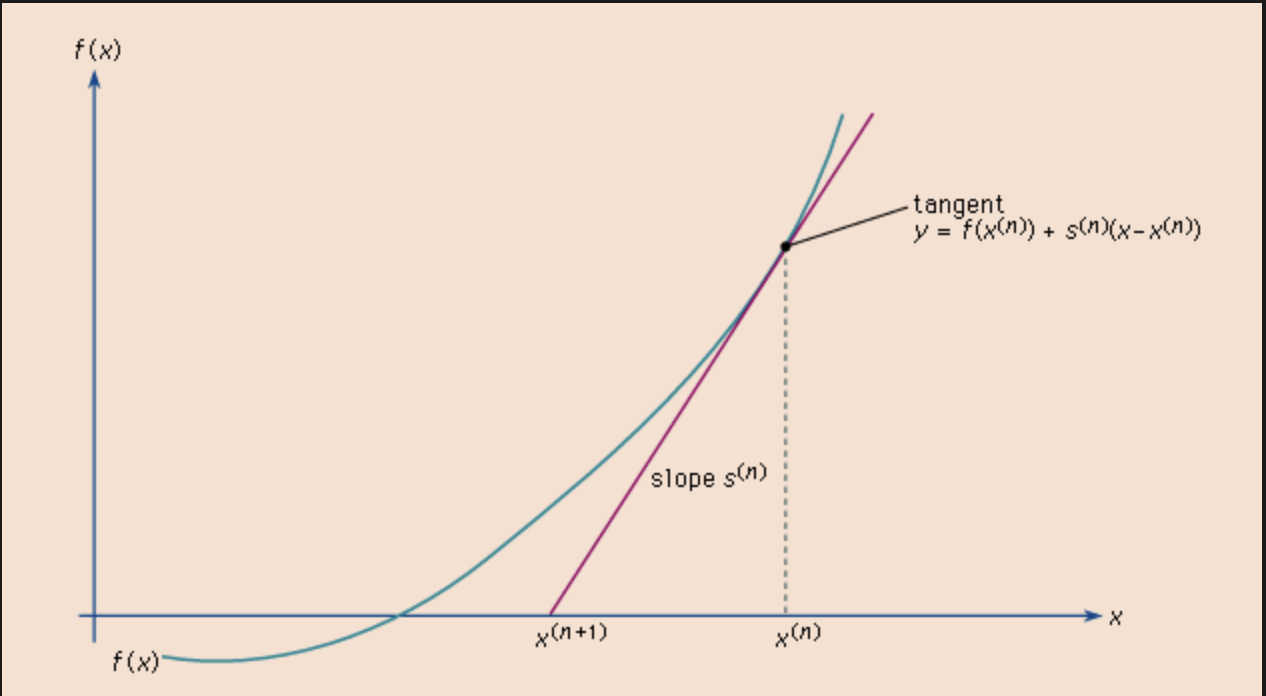
\includegraphics[width=\linewidth]{newton}\\[1mm]
\vspace{-1mm}
\small
\[
  x_{n+1}=x_n-\frac{f(x_n)}{f'(x_n)},
  \qquad
  e_{n+1}\approx \frac{f''}{2f'}\,e_n^{2},
\]
\footnotesize
so the error is \textbf{squared} each step --- the number of correct digits doubles. Cost: one $f$ \emph{and} one $f'$ per iteration.
\end{column}
\begin{column}{0.46\textwidth}
\begin{cautionbox}[title=\textbf{Three ways it goes wrong}]\footnotesize
$f'(x_n)\approx0$ sends the next iterate to infinity $\cdot$ a bad start converges to a different root, or to none $\cdot$ it will happily leave the economically sensible region, as it did on the hook slide.
\end{cautionbox}
\medskip
\begin{examplebox}\footnotesize
The standard repair is \textbf{damping}: take $x_{n+1}=x_n-\theta f/f'$ with $\theta\in(0,1]$, backtracking on $\theta$ until $|f|$ actually falls.
\end{examplebox}
\end{column}
\end{columns}
\vspace{1mm}
\src{Figure \texttt{newton.png} and the quadratic-convergence discussion from QM \emph{Numerical Methods}, Newton block, copied in.}
\end{frame}

%=============================================================================
\begin{frame}{Secant and Brent: Newton Without the Derivative}
\begin{columns}[T]
\begin{column}{0.52\textwidth}
\small
\textbf{Secant.} Replace $f'(x_n)$ by the slope through the last two points:
\[
  x_{n+1}=x_n-f(x_n)\frac{x_n-x_{n-1}}{f(x_n)-f(x_{n-1})} .
\]
One new evaluation per step, no derivative, and the order is the golden ratio
$\tfrac{1+\sqrt5}{2}\approx1.618$ --- slower than Newton per step, often faster per \emph{second}, because $f'$ is usually the expensive part.
\medskip

\textbf{Brent.} Keep a bracket, and inside it use inverse quadratic interpolation when that helps and bisection when it does not. Superlinear when the function is nice; never worse than bisection when it is not.
\end{column}
\begin{column}{0.45\textwidth}
\begin{takeawaybox}[title=\textbf{What was in the box}]\small
This is \texttt{brentq}. 3.A3 was entitled to trust it because we had \emph{proved} the residual crosses zero exactly once --- and a bracketing method with a valid bracket cannot fail.
\end{takeawaybox}
\medskip
\begin{examplebox}\footnotesize
The general rule: \textbf{bracket if you can, and only then go fast}. Every production solver is built this way.
\end{examplebox}
\end{column}
\end{columns}
\end{frame}

%=============================================================================
\begin{frame}{The Rates, Measured}
\begin{columns}[c]
\begin{column}{0.53\textwidth}
\centering
\begin{tikzpicture}
\begin{axis}[
    width=7.9cm, height=5.4cm, xmin=0, xmax=44, ymin=-16.5, ymax=1.5,
    xlabel={\scriptsize iteration $n$}, ylabel={\scriptsize $\log_{10}|x_n-x^{*}|$},
    tick label style={font=\scriptsize},
    axis x line*=bottom, axis y line*=left,
    legend style={font=\tiny, draw=none, fill=none, at={(0.98,0.97)}, anchor=north east}]
  \addplot[very thick, black!55] coordinates {(1,0.343) (2,-0.547) (3,-0.018) (4,-0.471) (5,-1.567) (6,-0.891) (7,-1.295) (8,-1.928) (9,-2.117) (10,-2.683) (11,-2.555) (12,-3.449) (13,-3.066) (14,-3.599) (15,-4.284) (16,-4.001) (17,-4.621) (18,-4.853) (19,-5.304) (20,-5.345) (21,-6.656) (22,-5.667) (23,-6.015) (24,-6.429) (25,-7.121) (26,-7.139) (27,-8.822) (28,-7.449) (29,-7.769) (30,-8.110) (31,-8.505) (32,-9.091) (33,-9.458) (34,-9.636) (35,-10.234) (36,-10.064) (37,-10.854) (38,-10.654) (39,-11.387) (40,-11.306) (41,-12.374) (42,-11.735) (43,-12.149) (44,-12.845) (45,-12.853) (46,-14.750) (47,-13.159) (48,-13.472) (49,-13.796) (50,-14.148) (51,-14.574) (52,-16.000)};
  \addlegendentry{bisection (order 1.04)}
  \addplot[very thick, orange!80!black, mark=square*, mark size=1.1pt] coordinates {(1,-0.360) (2,-0.930) (3,-1.968) (4,-3.581) (5,-6.230) (6,-10.492) (7,-16.000)};
  \addlegendentry{secant (1.61)}
  \addplot[very thick, RedTitle, mark=*, mark size=1.3pt] coordinates {(1,0.077) (2,-0.568) (3,-1.824) (4,-4.329) (5,-9.340) (6,-15.051)};
  \addlegendentry{Newton (2.00)}
\end{axis}
\end{tikzpicture}
\end{column}
\begin{column}{0.44\textwidth}
\small
Market clearing for $100p^{-0.5}=e^{0.5p}-1$, whose root is $p^{*}=7.2786$.
\medskip
\begin{center}\footnotesize
\begin{tabularx}{\linewidth}{@{}>{\raggedright\arraybackslash}X c c@{}}
\toprule
 & \textbf{to $10^{-12}$} & \textbf{order} \\
\midrule
bisection & 41 & 1.04 \\
secant & 7 & 1.61 \\
Newton & \textbf{6} & \textbf{2.00} \\
\bottomrule
\end{tabularx}
\end{center}
\vspace{1mm}
\begin{examplebox}\footnotesize
The observed orders are $1.04$, $1.61$ and $2.00$ against theoretical $1$, $1.618$ and $2$. The theory is not decoration --- it predicts the slopes on the left to two digits.
\end{examplebox}
\end{column}
\end{columns}
\vspace{1mm}
\src{Observed order estimated from the last clean error triple, $\log(e_{n+1}/e_n)/\log(e_n/e_{n-1})$. Bisection's error is not monotone, so that estimator is noisy for it; its rate is linear with ratio $1/2$ per step, which is the cleaner statement.}
\end{frame}

%=============================================================================
\begin{frame}{Systems: The Jacobian, and Why You Avoid Rebuilding It}
\begin{columns}[T]
\begin{column}{0.52\textwidth}
\small
For $F:\mathbb{R}^{N}\to\mathbb{R}^{N}$, Newton becomes
\[
  J(x_n)\,\Delta_n=-F(x_n), \qquad x_{n+1}=x_n+\Delta_n,
\]
with $J_{ij}=\partial F_i/\partial x_j$. Two costs, and the second is the one that hurts:
\begin{itemize}\footnotesize
  \item \textbf{building} $J$: $N^2$ partial derivatives, each needing an evaluation if done by finite differences;
  \item \textbf{solving} the linear system: $O(N^{3})$.
\end{itemize}
\medskip
\textbf{Broyden} updates an \emph{approximate} $J$ from the step it just took, so it builds a Jacobian once and never again.
\end{column}
\begin{column}{0.45\textwidth}
\begin{center}\footnotesize
\begin{tabularx}{\linewidth}{@{}>{\raggedright\arraybackslash}X c c@{}}
\toprule
$x^2+y^2=4$, $e^{x}+y=1$ & \textbf{iters} & \textbf{Jacobians} \\
\midrule
Newton & \textbf{5} & 5 \\
Broyden & 14 & \textbf{1} \\
\bottomrule
\end{tabularx}
\end{center}
\vspace{1mm}
\begin{takeawaybox}\footnotesize
Both reach a residual of $0$ to machine precision. Broyden takes nearly three times the iterations and one fifth of the derivative work --- and when $J$ is the expensive part, that is the trade you want.
\end{takeawaybox}
\end{column}
\end{columns}
\vspace{1mm}
\src{Cost accounting adapted from QM \emph{Numerical Methods}, ``Why Multivariate is Hard''. Where the derivatives come from is 4.A4.}
\end{frame}

%=============================================================================
\begin{frame}{Fixed Points, and the Cheapest Repair in Numerical Economics}
\begin{columns}[T]
\begin{column}{0.51\textwidth}
\small
Many equilibrium problems arrive as $x=g(x)$ and are solved by just iterating it. That converges only if $|g'(x^{*})|<1$, and in economics it frequently is not.
\medskip

\textbf{Damping} (relaxation) fixes it in one line:
\[
  x_{n+1}=(1-\theta)x_n+\theta\, g(x_n), \qquad \theta\in(0,1].
\]
The map's slope becomes $1-\theta+\theta g'$, so a small enough $\theta$ always pulls it inside the unit circle.
\end{column}
\begin{column}{0.46\textwidth}
\begin{center}\footnotesize
\begin{tabularx}{\linewidth}{@{}>{\raggedright\arraybackslash}X c@{}}
\toprule
$g(x)=4-x^{2}/4$ & \textbf{iterations} \\
\midrule
$\theta=1$ (no damping) & \textbf{diverges} \\
$\theta=0.5$ & \textbf{11} \\
$\theta=0.2$ & 41 \\
\bottomrule
\end{tabularx}
\end{center}
\vspace{1mm}
\begin{takeawaybox}\footnotesize
Undamped iteration never converges here. At $\theta=0.5$ it takes eleven steps. \textbf{Too small a $\theta$ is also a cost} --- $0.2$ needs four times as many.
\end{takeawaybox}
\medskip
\begin{examplebox}\footnotesize
This is exactly how the outer loop on $r$ in Aiyagari is stabilised (S6).
\end{examplebox}
\end{column}
\end{columns}
\end{frame}

%=============================================================================
\begin{frame}{Four Checks Before You Believe a Root}
\begin{columns}[T]
\begin{column}{0.50\textwidth}
\small
\begin{enumerate}\footnotesize
  \item \textbf{Did it converge?} Read the solver's own flag --- do not assume. Both failures on the hook slide reported a number.
  \item \textbf{Is the residual small?} $|f(x)|<$ tol, checked by you, in the units of the problem.
  \item \textbf{Is it feasible?} A negative price or a negative consumption is not a solution, whatever the residual says.
  \item \textbf{Is it unique?} Re-solve from twenty different starts and count the distinct answers.
\end{enumerate}
\end{column}
\begin{column}{0.47\textwidth}
\begin{cautionbox}[title=\textbf{The failure mode to know}]\footnotesize
The notebook on the hook slide printed a \texttt{\checkmark} next to both wrong answers, because the tick was hard-coded rather than read off \texttt{result.converged}. It then \emph{validated} $p=245$ as the equilibrium.
\end{cautionbox}
\medskip
\begin{takeawaybox}\footnotesize
Check 4 is the one people skip, and it is the one that matters in economics: \textbf{multiple equilibria are a result, not a bug} --- but only if you looked.
\end{takeawaybox}
\end{column}
\end{columns}
\vspace{1mm}
\src{The four-check validator is adapted from QM \emph{Numerical Methods, Research Architect}, Part III.}
\end{frame}

%=============================================================================
\begin{frame}{Takeaways}
\begin{takeawaybox}
\begin{itemize}\small
  \item Every fixed point in this course is a root-finding problem, and \texttt{brentq} is no longer a black box: it is \textbf{a bracket with a fast method inside it}.
  \item The rates are real and we measured them --- observed orders $1.04$, $1.61$ and $2.00$ against theoretical $1$, $1.618$ and $2$. Newton reached $10^{-12}$ in \textbf{six} iterations; bisection took 41.
  \item Speed and safety trade off exactly as the theory says. \textbf{Bracket if you can}, then go fast inside the bracket.
  \item In systems, the Jacobian is the expense. Broyden pays three times the iterations for one fifth of the derivative work.
  \item A solver that returns a number has not told you it is right. \textbf{Read the convergence flag, check the residual, check feasibility, and look for other roots.}
\end{itemize}
\end{takeawaybox}
\end{frame}

%=============================================================================
\begin{frame}{Bridge: The Other Half of the Inner Loop}
\begin{columns}[T]
\begin{column}{0.52\textwidth}
\small
Time iteration needed a root per grid point, and we have now opened that box. But 3.A2 and 3.A4 had a different inner loop: a \textbf{maximization}, done by searching all $N$ candidates on the grid --- and it left a staircase in the policy that no amount of iterating removed.
\medskip

Maximizing is not the same problem as root-finding, and the safe-versus-fast trade-off comes back in a different shape: without derivatives, the analogue of bisection is not halving an interval but shrinking it by a very particular ratio.
\end{column}
\begin{column}{0.45\textwidth}
\begin{conceptbox}[title=\textbf{Next (4.A2)}]\small
Optimization on an interval: golden section, why the ratio is golden, and Brent's minimizer.\\[1mm]
Then the pay-off --- the 3.A4 staircase retired, and what continuous choice actually bought us.
\end{conceptbox}
\end{column}
\end{columns}
\end{frame}

\end{document}
